\documentclass[journal,twoside]{IEEEtran}
\usepackage{amsmath}
\interdisplaylinepenalty=2500
\usepackage[dvips]{graphicx}
\newtheorem{definition}{Definition}

\begin{document}
\bibliographystyle{IEEEtran.bst}

\title{Symbolic Circuit Modeling and Simulation\\
Using a Sparse Matrix: An Introduction}
\author{John Rugis
\thanks{The author is with the Department of Electrical and Computer Engineering at Manukau Institute of Technology in Auckland, New Zealand.}}
\markboth{Article Preprint: January 2004 (rev 06/04)}{Rugis: Symbolic Circuit Modeling and Simulation}
\maketitle


\begin{abstract}
The first part of this article introduces some basic concepts and briefly contrasts electronic circuit modeling with circuit analysis. Then a sparse matrix generalized circuit model is built from first principles by means of an example. Finally, examples of symbolic modeling and simulation for the purposes of theorem development and circuit design validity checking are presented. Note that in this article we will be considering linear circuit elements only.
\end{abstract}

\section{Introduction}
\PARstart{W}{e} begin with the question: 
\emph{What is an is an electronic circuit?}
An electronic circuit is a collection of interconnected electronic components that has well-defined deterministic functionality when it is \emph{running}.
The functionality of a circuit when it is running is fully characterized by

\begin{enumerate}
\item the electric current through each component,
\item the voltage drop across each component,
\item and the voltage potential at each of the interconnections with respect to an arbitrary \emph{ground} interconnection.
\end{enumerate}
Each of the voltages has a polarity and each of the currents has a direction and can thus be either positive or negative.

A circuit is often thought of as a system having one or more \emph{inputs} and one or more \emph{outputs}. When we say that a circuit is \emph{running} what we mean is that it's inputs and outputs are (possibly constant) functions of time.

When a collection of interconnected circuit elements does not have well-defined deterministic functionality we say that the circuit design is not \emph{valid}.\\

\emph{What is circuit modeling?}\\
The modeling of electronic circuits consists of producing a mathematical representation of the circuit and all of it's characteristics.
Circuit models are an abstraction of their real-world counterpart and as such use \emph{idealized} versions of real physical components and their interconnections.
The modeling process is made easier by intentionally omitting any real-world considerations that are not of immediate interest eg. temperature effects.

Any complete circuit model includes variables for each of the circuit's characteristic currents and voltages. 
\emph{Inputs} are modeled using (possibly additional) circuit components and \emph{outputs} are modeled as one or more of the characteristic currents or voltages.
Circuit models are used by circuit designers to gain insight into the functioning of circuits and as an aid in the circuit design process.

We point out that circuit modeling is not the same thing as circuit analysis.
Circuit analysis typically consists of applying a sequence of simplification methods one after the other until the answer to some specific question about the circuit's functionality has been reduced to the obvious.
Circuit analysis can be characterized by saying that is done using a collection of tools and an \emph{as needed} approach.
This \emph{analysis by simplification} has the limitation that we can ask only one question at a time about the circuit.
   
Modeling on the other hand can answer all questions about the functioning of any given circuit \emph{simultaneously}. 
Modeling is best done with methods that seek comprehensive generalized representation.

Models are mostly used for simulation.
Simulation means that we run the model, often but not necessarily  on a computer, and that the model behaves like the actual physical circuit.
It is reasonable to expect that a circuit model will give us some indication when a circuit design is not valid.\\ 

\emph{Is it possible to model a linear circuit with a single equation?}\\
Yes! It is possible to model any given linear circuit, no matter how complex,  with a single matrix algebraic equation \cite{lc:lnc,jv:cm}.

\section{A generalized circuit model}
We will use an example and proceed step-by-step from first principles to construct a sparse matrix  \cite{gh:st} generalized model.
\subsection{Schematic diagram}
Figure~\ref{fig:sch} shows a schematic diagram of a simple circuit that contains three components (a constant independent voltage source and two resistors) plus ground.
Schematics are the standard representation commonly used by circuit designers to specify electronic circuits.
Note that some components, such as the resistors, can be connected in either direction without effecting the functionality of the circuit. 
Other components, such as the independent voltage source, have a polarity and reversal changes the functionality of the circuit.

\begin{figure}[h]
\centering
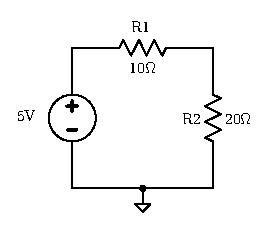
\includegraphics{c1}
\caption{Schematic of a simple circuit.}
\label{fig:sch}
\end{figure}

A schematic diagram can be used as an unambiguous guide for building a real physical circuit and as such is a complete circuit specification.
But the schematic diagram alone is not sufficient for circuit modeling.

\subsection{Digraph}
Digraphs, taken from the mathematics subject area known as graph theory, can be used to represent circuits somewhat more abstractly.  
Figure~\ref{fig:dig} shows a digraph representation of the same simple circuit.

\begin{figure}[h]
\centering
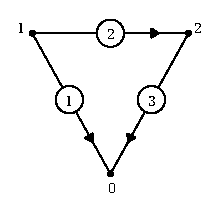
\includegraphics{c2}
\caption{A circuit digraph.}
\label{fig:dig}
\end{figure}

This digraph has three \emph{nodes} which are shown as labeled dots, and three \emph{branches} shown as line segments with labeled circles on them.
Additionally, each branch has a small arrowhead that indicates an associated reference direction pointing from it's \emph{source node} to it's \emph{destination node}.
Note that each branch corresponds to a circuit component and that the nodes correspond to interconnections.

The labeling and reference directions provide the additional information required for modeling the circuit.
The digraph highlights the circuit's interconnection topology and the reference directions but omits the component types, component values, and any possible component polarity.

\subsection{Netlist}
Another circuit representation, as used by the Spice \cite{uoc:spice} circuit simulation program, is a circuit netlist.
The netlist is a non-graphical text-only representation.
Here is one possible netlist for the same circuit:\\[10pt]
\texttt{V1 1 0 5\\
R1 1 2 10\\
R2 2 0 20\\}\\
The format for each line in this netlist is:
\begin{enumerate}
\item Branch label with the first character indicating component type.
\item Source node label.
\item Destination node label.
\item Numeric component value.\\
\end{enumerate}
There are a number of conventions that are followed both with netlists and circuit digraphs:
\begin{enumerate}
\item The ground node is always named 0.
\item All of the other node labels as well as all of the branch labels are arbitrary.
\item A positive numeric value for branch current indicates that (positive) current is flowing from the source node to the destination node, whereas a negative numeric value indicates that the current is in fact flowing in the opposite direction.
\item A positive numeric value for branch voltage indicates that voltage drops when moving from the source node to the destination node,  whereas a negative numeric value indicates that voltage actually drops in the opposite direction.
\end{enumerate}

The netlist is a complete circuit specification that can be used as a basis for modeling. The netlist is also conveniently computer readable.

\subsection{Incidence matrix.} The first step in producing a mathematical circuit representation is to construct a node-branch incidence matrix for the circuit.
The purpose of this matrix $\mathbf{A}_a$ is to capture the circuit's interconnection topology.

For a circuit with $n$ nodes and $b$ branches we start with a zero matrix having $n$ rows and $b$ columns.
Then for each branch column we put a `1' in the corresponding source node row and `-1' in the corresponding destination node row.
The result for the sample circuit is given by:
\begin{equation}
\mathbf{A}_a
=\;\;
\begin{array}{cc}
\begin{matrix}
n_0\\
n_1\\
n_2
\end{matrix}
&
\begin{bmatrix}
-1 &0 &-1\\
1 &1 &0\\
0 &-1 &1
\end{bmatrix}\\
&b_1\text{\hspace{15pt}}b_2\text{\hspace{15pt}}b_3
\end{array}
\end{equation}

Because the voltage potential at the ground node is always zero, a reduced incidence matrix $\mathbf{A}$, in which the ground node row has been deleted, is ultimately no less informative.
The reduced incidence matrix for the sample circuit is:
\begin{equation*}
\mathbf{A}
=
\begin{bmatrix}
1 &1 &0\\
0 &-1 &1
\end{bmatrix}
\end{equation*}
The dimensions of $\mathbf{A}$ are $(n-1)\times b$ where $n$ is the number of nodes and $b$ is the number of branches.

\subsection{Kirchhoff's's Current Law}
Kirchhoff's's Current Law states that \textit{the algebraic sum of currents leaving any node is zero}.

For the sample circuit, KCL involves all three branch currents $i_1, i_2, i_3$ and applies to all three interconnection nodes $n_0, n_1, n_2$ resulting in the following equations:
\begin{align*}
-i_1-i_3 &= 0\\
i_1 + i_2 &= 0\\
-i_2 + i_3 &= 0
\end{align*}
These equations can be rewritten in terms of the circuit's incidence matrix and a column vector of branch currents as follows:
\begin{equation*}
\begin{bmatrix}
-1 &0 &-1\\
1 &1 &0\\
0 &-1 &1
\end{bmatrix}
\begin{bmatrix}
i_1\\i_2\\i_3
\end{bmatrix}
=
\begin{bmatrix}
0\\0\\0
\end{bmatrix}
\end{equation*}
In general, KCL can be expressed in matrix form as $\mathbf{A}_a\mathbf{i}=\mathbf{0}$ and when using the reduced incidence matrix as
\begin{equation}
\mathbf{A}\mathbf{i}=\mathbf{0}\label{eq:kcl}
\end{equation}
where $\mathbf{i}$ is a column vector of branch currents and $\mathbf{0}$ is a column vector of zeros.

\subsection{Kirchhoff's's Voltage Law}
Kirchhoff's's Voltage Law in one of it's most general forms states that \textit{the voltage drop between any two nodes is equal to the difference of the two node voltages}.

For the sample circuit, KVL involves three branch voltage drops $v_1, v_2, v_3$ and three node voltages $e_0, e_1, e_2$. Remembering that $e_0 = 0$ this results in the following equations:
\begin{align*}
v_1 &= e_1 - 0\\
v_2 &= e_1 - e_2\\
v_3 &= e_2 - 0
\end{align*}
These equations can be rewritten in matrix form using the transpose of the circuit's reduced incidence matrix as follows:
\begin{equation*}
\begin{bmatrix}
v_1\\v_2\\v_3
\end{bmatrix}
=
\begin{bmatrix}
1 &0\\
1 &-1\\
0 &1
\end{bmatrix}
\begin{bmatrix}
e_1\\e_2
\end{bmatrix}
\end{equation*}
In general, KVL can be expressed in matrix form as
\begin{equation}
\mathbf{v}=\mathbf{A}^T\mathbf{e}\label{eq:kvl}
\end{equation}
where $\mathbf{v}$ is a column vector of branch voltages and $\mathbf{e}$ is a column vector of node voltages.

KCL (\ref{eq:kcl}) and KVL (\ref{eq:kvl}) can be combined into the single equation
\begin{equation}
\begin{bmatrix}
\mathbf{0} &\mathbf{0} &\mathbf{A}\\
-\mathbf{A}^T &\mathbf{1} &\mathbf{0}
\end{bmatrix}
\begin{bmatrix}
\mathbf{e}\\
\mathbf{v}\\
\mathbf{i}
\end{bmatrix}
=
\begin{bmatrix}
\mathbf{0}\\
\mathbf{0}\\
\end{bmatrix}
\end{equation}
where $\mathbf{1}$ is an identity matrix and $\mathbf{0}$ is a zero matrix having the requisite dimensions.
Note that this single equation encodes all of the circuit's component interconnections, as well as both KCL and KVL, and holds true for all circuits.
What's needed to finish off the model formulation is additional specific component type information.

\subsection{Component Characteristics.}
A component's type defines a characteristic $vi$ relationship for each branch.
The $vi$ relationship for resistors is $v_b=i_bR$ where $R$ is the resistor's \emph{resistance}.
For an independent voltage source whose voltage is $V$ the relationship is $v_b=V$ no matter what $i_b$ is.
For the sample circuit:
\begin{align*}
v_1&=5\\
v_2&=10\;i_2\\
v_3&=20\;i_3
\end{align*}
These equations can each be rearranged to take the form: 
\begin{equation*}
av_b+bi_b=u_b
\end{equation*}
For the sample circuit we now have:
\begin{align*}
v_1=5\\
v_2-10\;i_2=0\\
v_3-20\;i_3=0
\end{align*}
These equations can be combined and rewritten in matrix form:
\begin{equation*}
\begin{bmatrix}
1 &0 &0\\
0 &1 &0\\
0 &0 &1
\end{bmatrix}
\begin{bmatrix}
v_1\\v_2\\v_3
\end{bmatrix}
+
\begin{bmatrix}
0 &0 &0\\
0 &-10 &0\\
0 &0 &-20
\end{bmatrix}
\begin{bmatrix}
i_1\\i_2\\i_3
\end{bmatrix}
=
\begin{bmatrix}
5\\0\\0
\end{bmatrix}
\end{equation*}
In general the characteristic equations for all \emph{linear resistive components} can be combined and written in the form 
\begin{equation}
\mathbf{Mv}+\mathbf{Ni}=\mathbf{u}_s\label{eq:cc}
\end{equation}
where $\mathbf{M}$ is an array of voltage coefficients, $\mathbf{N}$ is an array of current coefficients, and $\mathbf{u_s}$ is a column vector of independent source magnitudes.
The dimensions of both $\mathbf{M}$ and $\mathbf{N}$ are $b\times b$ where $b$ is the number of branches.

\subsection{Sparse Matrix Model.}
Now (\ref{eq:kcl}), (\ref{eq:kvl}), and (\ref{eq:cc}) can all be combined giving:
\begin{equation}
\begin{bmatrix}
\mathbf{0} &\mathbf{0} &\mathbf{A}\\
-\mathbf{A}^T &\mathbf{1} &\mathbf{0}\\
\mathbf{0} &\mathbf{M} &\mathbf{N}
\end{bmatrix}
\begin{bmatrix}
\mathbf{e}\\
\mathbf{v}\\
\mathbf{i}
\end{bmatrix}
=
\begin{bmatrix}
\mathbf{0}\\
\mathbf{0}\\
\mathbf{u}_s
\end{bmatrix}\label{eq:st}
\end{equation}
Equation (\ref{eq:st}) is a \emph{sparse matrix} generalized circuit model for linear resistive circuits.
This sparse matrix equation is a complete model in that it encodes all of the circuit's component characteristics and interconnections as well as both KCL and KVL.
Note that the sparse matrix equation has the form
\begin{equation}
\mathbf{Tw}=\mathbf{u}\label{eq:stf}
\end{equation}
where $\mathbf{T}$ is a square matrix with dimensions $(n-1)2b$ where the circuit that it represents has $n$ nodes and $b$ branches.

In most circuit simulation applications one or more of the entries in $\mathbf{u}$ are the circuit's \emph{inputs}, one or more of the the entries in $\mathbf{w}$ are the circuit's \emph{outputs}, and the entries in $\mathbf{T}$ are constants.
Running a simulation means that we find the solution $\mathbf{w}$ to equation (\ref{eq:stf}).\\

The complete sparse matrix equation for the sample circuit is:
\begin{equation*}
\left[\begin{array}{cc|ccc|ccc}
0 &0 &0 &0 &0 &1 &1 &0\\
0 &0 &0 &0 &0 &0 &-1 &1\\ \hline
-1 &0 &1 &0 &0 &0 &0 &0\\
-1 &1 &0 &1 &0 &0 &0 &0\\
0 &-1 &0 &0 &1 &0 &0 &0\\ \hline
0 &0 &1 &0 &0 &0 &0 &0\\
0 &0 &0 &1 &0 &0 &-10 &0\\
0 &0 &0 &0 &1 &0 &0 &-20
\end{array}\right]
\left[\begin{array}{c}
e_1\\e_2\\ \hline
v_1\\v_2\\v_3\\ \hline
i_1\\i_2\\i_3
\end{array}\right]
=
\left[\begin{array}{c}
0\\0\\ \hline
0\\0\\0\\ \hline
5\\0\\0
\end{array}\right]
\end{equation*}
Gaussian elimination and exact arithmetic yields the solution
\begin{equation*}
\left[\begin{array}{c}
e_1\\e_2\\ \hline
v_1\\v_2\\v_3\\ \hline
i_1\\i_2\\i_3
\end{array}\right]
=
\left[\begin{array}{c}
5\\10/3\\ \hline
5\\5/3\\10/3\\ \hline
-1/6\\1/6\\1/6
\end{array}\right]
\end{equation*}
which fully characterizes the sample circuit when it is running.

\subsection{Symbolic Modeling and Simulation.} The sparse matrix circuit model equation can also be solved using symbolic rather than numerical component values.
For the sample circuit we have:
\begin{equation*}
\left[\begin{array}{cc|ccc|ccc}
0 &0 &0 &0 &0 &1 &1 &0\\
0 &0 &0 &0 &0 &0 &-1 &1\\ \hline
-1 &0 &1 &0 &0 &0 &0 &0\\
-1 &1 &0 &1 &0 &0 &0 &0\\
0 &-1 &0 &0 &1 &0 &0 &0\\ \hline
0 &0 &1 &0 &0 &0 &0 &0\\
0 &0 &0 &1 &0 &0 &-R_1 &0\\
0 &0 &0 &0 &1 &0 &0 &-R_2
\end{array}\right]\!\!
\left[\begin{array}{c}
e_1\\e_2\\ \hline
v_1\\v_2\\v_3\\ \hline
i_1\\i_2\\i_3
\end{array}\right]
\!=\!
\left[\begin{array}{c}
0\\0\\ \hline
0\\0\\0\\ \hline
V_1\\0\\0
\end{array}\right]
\end{equation*}
Symbolic Gaussian elimination yields the solution:
\begin{equation*}
\left[\begin{array}{c}
e_1\\e_2\\ \hline
v_1\\v_2\\v_3\\ \hline
i_1\\i_2\\i_3
\end{array}\right]
=
\left[\begin{array}{c}
V_1\\V_1R_2/(R_1+R_2)\\ \hline
V_1\\V_1R_1/(R_1+R_2)\\V_1R_2/(R_1+R_2)\\ \hline
-V_1/(R_1+R_2)\\V_1/(R_1+R_2)\\V_1/(R_1+R_2)
\end{array}\right]
\end{equation*}
Note the richness of this solution in that it effectively includes both the series resistor formula and the voltage divider equation:
\begin{eqnarray*}
R_{total}&=&-(v_1/i_1)=R_1+R_2\\
e_2&=&V_1R_2/(R_1+R_2)
\end{eqnarray*}

\subsection{Circuit Design Validity Checking.} Recall that, by definition, a circuit has well-defined deterministic functionality. 
What we mean by a \emph{valid circuit design} is that it in fact represents a circuit having the required well-defined functionality. 
In terms of the model what this means is that equation (\ref{eq:st}) has a well-defined unique solution.
A fundamental result from linear algebra states that all equations of the form given by (\ref{eq:stf}) have either
\begin{enumerate}
\item a single solution,
\item no solution,
\item or infinitely many solutions.
\end{enumerate}
Thus, \emph{a circuit design is valid if and only if it's model has a single solution.} With this in mind, we are now in a position to explore a number of example circuit designs for validity.\\ 

\subsubsection{Circuit design example}
Is the single independent voltage source shown in Figure \ref{fig:ex1} a valid circuit design?

\begin{figure}[h]
\centering
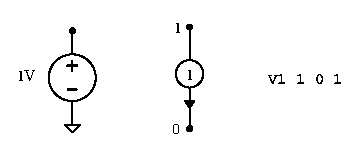
\includegraphics{c3}
\caption{Schematic, digraph, and netlist.}
\label{fig:ex1}
\end{figure}

Working with the circuit model in the form of an augmented matrix and using symbolic Gaussian elimination gives the following result:
\begin{equation*}
\left[\begin{array}{ccc|c}
0 &0 &1 &0\\
-1 &1 &0 &0\\
0 &1 &0 &V_1
\end{array}\right]
=
\left[\begin{array}{ccc|c}
1 &0 &0 &V_1\\
0 &1 &0 &V_1\\
0 &0 &1 &0
\end{array}\right]
\end{equation*}
Which means that the solution is:
\begin{equation*}
\left[\begin{array}{c}
e_1\\
v_1\\ 
i_1
\end{array}\right]
=
\left[\begin{array}{c}
V_1\\
V_1\\
0
\end{array}\right]
\end{equation*}
All of the circuit's characteristics are well-defined, therefore this circuit design is valid.

\subsubsection{Circuit design example}
Is the single independent current source shown in Figure \ref{fig:ex2} a valid circuit?

\begin{figure}[h]
\centering
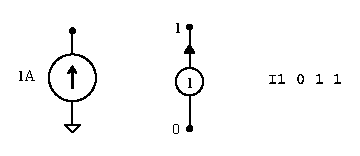
\includegraphics{c4}
\caption{Schematic, digraph, and netlist.}
\label{fig:ex2}
\end{figure}

The augmented matrix and symbolic Gaussian elimination gives the result:
\begin{equation*}
\left[\begin{array}{ccc|c}
0 &0 &-1 &0\\
1 &1 &0 &0\\
0 &0 &1 &I_1
\end{array}\right]
=
\left[\begin{array}{ccc|c}
1 &1 &0 &0\\
0 &0 &0 &0\\
0 &0 &1 &0
\end{array}\right]
\end{equation*}
This means that there are an infinite number of solutions as long as the following conditions are met:
\begin{equation*}
\left[\begin{array}{c}
e_1+v_1\\
i_1
\end{array}\right]
=
\left[\begin{array}{c}
0\\
0
\end{array}\right]
\end{equation*}
The circuit's characteristics are not uniquely determined, therefore this circuit design is not valid.

\subsubsection{Circuit design example}
Is the single resistor as shown in Figure \ref{fig:ex3} a valid circuit?

\begin{figure}[h]
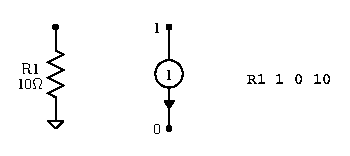
\includegraphics{c5}
\centering
\caption{Schematic, digraph, and netlist.}
\label{fig:ex3}
\end{figure}

The augmented matrix and symbolic Gaussian elimination gives the result:
\begin{equation*}
\left[\begin{array}{ccc|c}
0 &0 &1 &0\\
-1 &1 &0 &0\\
0 &1 &-R_1 &0
\end{array}\right]
=
\left[\begin{array}{ccc|c}
1 &0 &0 &0\\
0 &1 &0 &0\\
0 &0 &1 &0
\end{array}\right]
\end{equation*}
Which means that the solution is:
\begin{equation*}
\left[\begin{array}{c}
e_1\\
v_1\\ 
i_1
\end{array}\right]
=
\left[\begin{array}{c}
0\\
0\\
0
\end{array}\right]
\end{equation*}
All of the circuit's characteristics are well-defined, therefore this circuit design is valid.

\subsubsection{Circuit design example}
Do the two resistors as shown in Figure \ref{fig:ex4} form a valid circuit?

\begin{figure}[h]
\centering
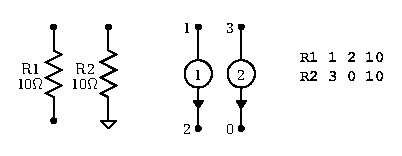
\includegraphics{c6}
\caption{Schematic, digraph, and netlist.}
\label{fig:ex4}
\end{figure}
We start with the augmented matrix:
\begin{equation*}
\left[\begin{array}{ccccccc|c}
0 &0 &0 &0 &0 &1 &0 &0\\
0 &0 &0 &0 &0 &-1 &0 &0\\
0 &0 &0 &0 &0 &0 &1 &0\\
-1 &1 &0 &1 &0 &0 &0 &0\\
0 &0 &-1 &0 &1 &0 &0 &0\\
0 &0 &0 &1 &0 &-R_1 &0 &0\\
0 &0 &0 &0 &1 &0 &-R_2 &0\\
\end{array}\right]
\end{equation*}
Symbolic Gaussian elimination gives the result:
\begin{equation*}
\left[\begin{array}{ccccccc|c}
1 &-1 &0 &0 &0 &0&0 &0\\
0 &0 &1 &0 &0 &0 &0 &0\\
0 &0 &0 &1 &0 &0 &0 &0\\
0 &0 &0 &0 &1 &0 &0 &0\\
0 &0 &0 &0 &0 &1 &0 &0\\
0 &0 &0 &0 &0 &0 &1 &0\\
0 &0 &0 &0 &0 &0 &0 &0\\
\end{array}\right]
\end{equation*}
Which means that the solution is:
\begin{equation*}
\left[\begin{array}{c}
e_1-e_2\\
e_3\\
v_1\\ 
v_2\\ 
i_1\\
i_2
\end{array}\right]
=
\left[\begin{array}{c}
0\\
0\\
0\\
0\\
0\\
0
\end{array}\right]
\end{equation*}
The circuit's characteristics are not uniquely determined as either $e_1$ or $e_2$ could be a free variable, taking any value as long as the condition $e_1- e_2=0$ is met. Therefore this circuit design is not valid.
 
\subsubsection{Circuit design example}
Is the circuit design shown in Figure \ref{fig:ex5} valid?

\begin{figure}[h]
\centering

\includegraphics{c7}
\caption{Schematic, digraph, and netlist.}
\label{fig:ex5}
\end{figure}

We start with the augmented matrix
\begin{equation*}
\left[\begin{array}{cccccccc|c}
0 &0 &0 &0 &0 &-1 &1 &0 &0\\
0 &0 &0 &0 &0 &0 &-1 &1 &0\\
1 &0 &1 &0 &0 &0 &0 &0 &0\\
-1 &1 &0 &1 &0 &0 &0 &0 &0\\
0 &-1 &0 &0 &1 &0 &0 &0 &0\\
0 &0 &0 &0 &0 &1 &0 &0 &I_1\\
0 &0 &0 &0 &0 &0 &1 &0 &I_2\\
0 &0 &0 &0 &1 &0 &0 &-R_1 &0\\
\end{array}\right]
\end{equation*}
but after a number of elementary row operations the augmented matrix contains the row
\begin{equation*}
\left[\begin{array}{cccccccc|c}
0 &0 &0 &0 &0 &0 &0 &0 &I_1-I_2
\end{array}\right]
\end{equation*}
which indicates that when $I_1 \neq I_2$ there are no solutions and the circuit is thus not valid.
But what happens when the currents are equal?

Setting $I_2=I_1$ and continuing with Gaussian elimination leads to the result:
\begin{equation*}
\left[\begin{array}{cccccccc|c}
1 &0 &1 &0 &0 &0 &0 &0 &0\\
0 &1 &0 &0 &0 &0 &0 &0 &R_1I_1\\
0 &0 &1 &1 &0 &0 &0 &0 &-R_1I_1\\
0 &0 &0 &0 &1 &0 &0 &0 &R_1I_1\\
0 &0 &0 &0 &0 &1 &0 &0 &I_1\\
0 &0 &0 &0 &0 &0 &1 &0 &I_1\\
0 &0 &0 &0 &0 &0 &0 &1 &I_1\\
0 &0 &0 &0 &0 &0 &0 &0 &0\\
\end{array}\right]
\end{equation*}
The circuit's characteristics are still not uniquely determined as any one of $e_1$, $v_1$, or $v_2$ could be a free variable, the other two then being determined by: 
\begin{equation*}
\left[\begin{array}{c}
e_1+v_1\\
v_1+v_2
\end{array}\right]
=
\left[\begin{array}{c}
0\\
-R_1I_1
\end{array}\right]
\end{equation*}
Therefore there are no conditions under which this circuit design is valid.

\section{Conclusion.} A sparse matrix circuit model can be easily constructed from first principles and used with both numerical as well as symbolic component values. The utility of the model has been demonstrated in a number of ways. Carefully selected circuit simulations can yield fundamental circuit theorems. Symbolic Gaussian elimination applied to the model can be used to check circuits for design validity.

\section*{Acknowledgment}
This work was supported by a University Fellowship from Manukau Institute of Technology and by the Department of Mathematics at the University of Auckland.

\bibliography{circuit}

\vspace{20pt}
\flushleft
\copyright 2004 J. Rugis\\
email: jrugis@manukau.ac.nz\\

\end{document}